\documentclass[UTF8,fontset=fandol,aspectratio=169]{ctexbeamer}

\usetheme{Madrid}
\usecolortheme{default}
\setbeamertemplate{navigation symbols}{}
\setbeamertemplate{footline}[frame number]

\usepackage{booktabs}
\usepackage{tabularx}
\usepackage{graphicx}
\usepackage{tikz}
\usetikzlibrary{arrows.meta,positioning,shapes.geometric,fit}

\title[OpenClaw DeepResearch Evaluation]{OpenClaw 科研 Agent 的引用一致性评测}
\subtitle{实验架构、流程与工程经验}
\author{李佳蓓 \quad 马惠文 \quad 毛恺诚 \quad 陈思琪}
\date{\today}

\definecolor{mainblue}{RGB}{34,94,168}
\definecolor{accentgreen}{RGB}{42,137,89}
\definecolor{accentred}{RGB}{190,75,72}
\definecolor{softgray}{RGB}{245,247,250}

\tikzset{
  box/.style={
    rectangle,
    rounded corners=2pt,
    draw=mainblue,
    fill=softgray,
    align=center,
    minimum width=2.5cm,
    minimum height=0.85cm,
    font=\small
  },
  data/.style={
    cylinder,
    shape border rotate=90,
    aspect=0.25,
    draw=accentgreen,
    fill=green!6,
    align=center,
    minimum width=1.9cm,
    minimum height=0.9cm,
    font=\small
  },
  warn/.style={
    rectangle,
    rounded corners=2pt,
    draw=accentred,
    fill=red!5,
    align=center,
    minimum width=2.6cm,
    minimum height=0.8cm,
    font=\small
  },
  arrow/.style={-{Stealth[length=2.2mm]}, thick}
}

\begin{document}

\begin{frame}
  \titlepage
\end{frame}

\begin{frame}{项目目标}
  \begin{block}{核心问题}
    OpenClaw 搭建的科研 Agent 在生成科研报告时，是否会出现“引用与结论不一致”？
  \end{block}

  \vspace{0.3em}
  这里的“不一致”指：
  \begin{itemize}
    \item 报告中的结论看起来有引用支持；
    \item 但实际检查引用材料后，发现材料不能充分支持该结论；
    \item 严重时，引用材料甚至与结论相矛盾。
  \end{itemize}

  \vspace{0.3em}
  本项目不修改 Agent 内部代码，而是构造可复现的评测材料、运行脚本、日志和后续标注流程。
\end{frame}

\begin{frame}{被测系统：OpenClaw DeepResearch Agent}
  \begin{center}
  \begin{tikzpicture}[node distance=0.8cm and 1.0cm]
    \node[box] (prompt) {任务 Prompt\\五个科研主题};
    \node[box, right=of prompt] (agent) {OpenClaw Agent\\Deepseek v4 Pro};
    \node[box, right=of agent] (report) {科研报告\\带标准引用};

    \node[data, below=of prompt] (pdf) {PDF 材料\\\mbox{[A]-[C]}};
    \node[data, below=of agent] (tools) {Skills + MCP\\PDF / arxiv / refchecker};
    \node[data, below=of report] (memory) {Memory JSONL\\仅来自 repair log};

    \draw[arrow] (prompt) -- (agent);
    \draw[arrow] (agent) -- (report);
    \draw[arrow] (pdf) -- (agent);
    \draw[arrow] (tools) -- (agent);
    \draw[arrow] (report) -- (memory);
    \draw[arrow] (memory.west) to[bend right=16] (agent.south);
  \end{tikzpicture}
  \end{center}

  \vspace{0.2em}
  固定栈：OpenClaw + Deepseek v4 Pro + PDF skill + citation-standard skill + arxiv MCP + mcp-refchecker + Brave web search。
\end{frame}

\begin{frame}{Agent 生成的科研报告结构}
  \begin{columns}[T,onlytextwidth]
    \begin{column}{0.48\textwidth}
      \begin{block}{三段式结构化输出}
        \begin{enumerate}
          \setlength{\itemsep}{2pt}
          \item \textbf{总体评估} — 基于全部论文概括证据状况、共识/分歧、局限
          \item \textbf{逐条结论} — 5--8 条可证伪结论，每条带 CPS 出处标注
          \item \textbf{引用论文清单} — 完整元信息 + 检索策略
        \end{enumerate}
      \end{block}

      \begin{exampleblock}{逐条结论格式示例（C2 R1 实际输出）}
        \begin{quote}\footnotesize
          在纯合成数据替换式训练下，语言模型、扩散模型和 VAE 均必然出现 model collapse。\\
          \textbf{出处：}\texttt{[D] \S2.1::\P3}
        \end{quote}
      \end{exampleblock}
    \end{column}
    \begin{column}{0.48\textwidth}
      \begin{block}{输出 contract：四段 marker}
        \texttt{\# ORIGINAL\_REPORT}\\
        \hspace{1em}→ 阶段 1 初稿（三段式）\\
        \texttt{\# REFCHECKER\_REPAIR\_LOG}\\
        \hspace{1em}→ 阶段 2 JSONL 核查记录\\
        \texttt{\# REPAIRED\_REPORT}\\
        \hspace{1em}→ 阶段 3 修复后报告\\
        \texttt{\# RUN\_SUMMARY}\\
        \hspace{1em}→ 运行元数据
      \end{block}

      \begin{alertblock}{评测切入点}
        上述四个 marker 使输出可被程序拆解：\\
        \textbf{逐条抓取 claim + citation → 进入标注与统计流水线}
      \end{alertblock}
    \end{column}
  \end{columns}
\end{frame}

\begin{frame}{五个 Case 的设计}
  \begin{tabularx}{\textwidth}{@{}lX@{}}
    \toprule
    Case & 主题方向 \\
    \midrule
    C1 & 工具增强 LLM agent 与复杂 coding task \\
    C2 & 递归合成数据、弱数据、多模态合成训练、model collapse \\
    C3 & 蛋白-配体 docking、分子生成、binding affinity、benchmark leakage \\
    C4 & 人类认知 benchmark、多模态推理、cross-scene hallucination \\
    C5 & AI coding tools、experienced developer productivity、SWE-Bench Pro \\
    \bottomrule
  \end{tabularx}

  \vspace{0.8em}
  每个 case 固定提供部分文献，并要求 Agent 自主补充/使用相关材料生成报告。不同 case 覆盖不同学科和证据形态，避免只测单一 topic。
\end{frame}

\begin{frame}{引用标准化：citation-standard skill}
  \begin{columns}[T,onlytextwidth]
    \begin{column}{0.48\textwidth}
      \begin{block}{CPS 语法（Citation Position Standard）}
        \begin{itemize}
          \setlength{\itemsep}{3pt}
          \item 标签：\texttt{[A]}～\texttt{[F]} \quad 位置：\texttt{\S4.1::\P2}
          \item 元素：\texttt{::paragraph} / \texttt{::T2} / \texttt{::F1} / \texttt{::Eq}
          \item 多位置用 \texttt{;} 分隔
        \end{itemize}
      \end{block}

      \begin{block}{解决的问题}
        \begin{itemize}
          \setlength{\itemsep}{1pt}
          \item \texttt{Abstract} → 粒度太粗，多段落无法定位
          \item \texttt{第5页第3段} → 计数规则不统一
          \item \texttt{limitations 部分} → 自由文本无法解析
        \end{itemize}
      \end{block}
    \end{column}
    \begin{column}{0.48\textwidth}
      \begin{block}{技能组成}
        \begin{enumerate}
          \setlength{\itemsep}{2pt}
          \item \texttt{SKILL.md} — Agent 运行时遵守
          \item \texttt{cps-spec.md} — 完整语法规范
          \item \texttt{validate.py} — 合规检查脚本
        \end{enumerate}
      \end{block}
      \begin{block}{为什么需要}
        引用不统一 → \alert{人工标注和脚本检查不可复现}。CPS 用封闭词汇表 + 固定语法，每个 claim-citation pair 可被程序拆解。
      \end{block}
    \end{column}
  \end{columns}

\end{frame}

\begin{frame}{整体实验流程}
  \begin{center}
  \begin{tikzpicture}[node distance=0.65cm]
    \node[box] (prep) {准备 case\\PDF + prompt};
    \node[box, right=of prep] (orig) {生成\\ORIGINAL\_REPORT};
    \node[box, right=of orig] (check) {调用 refchecker\\+ 读原文核查};
    \node[box, right=of check] (repair) {生成\\REPAIRED\_REPORT};

    \node[data, below=of check] (log) {REFCHECKER\\REPAIR\_LOG};
    \node[data, below=of repair] (mem) {active\\memory.jsonl};

    \draw[arrow] (prep) -- (orig);
    \draw[arrow] (orig) -- (check);
    \draw[arrow] (check) -- (repair);
    \draw[arrow] (check) -- (log);
    \draw[arrow] (log) -- (mem);
    \draw[arrow] (mem) to[bend right=20] (prep.south);
  \end{tikzpicture}
  \end{center}

  \vspace{0.4em}
  输出 contract 固定为四段：\texttt{ORIGINAL\_REPORT}、\texttt{REFCHECKER\_REPAIR\_LOG}、\texttt{REPAIRED\_REPORT}、\texttt{RUN\_SUMMARY}。
\end{frame}

\begin{frame}{工具预实验 1：arxiv MCP}
  \begin{block}{目的}
    测试 Agent 能否自主找到合适的 [D][E][F] 三篇论文，而不是只依赖预置 PDF。
  \end{block}

  \begin{itemize}
    \item 条件：\texttt{arxiv\_off} vs \texttt{arxiv\_on}
    \item 规模：5 cases $\times$ 2 conditions $\times$ 3 runs
    \item 每个 run 记录 Agent 选择的三篇论文
    \item 标注维度：相关性、全文可得性、重复、是否偏题、是否有效
  \end{itemize}

  \vspace{0.4em}
  这个预实验的作用是证明 arxiv MCP 是否值得在后续主实验中固定开启。
\end{frame}

\begin{frame}{arxiv-MCP 贴合分数测试：核心发现}
  \begin{columns}[T,onlytextwidth]
    \begin{column}{0.45\textwidth}
      \begin{alertblock}{关键发现}
        arxiv-MCP 开关与论文贴合度并无显著相关性。\\
        大部分开启时贴合得分反而略低于 off。
      \end{alertblock}
      \begin{block}{最值得关注的异常}
        \textbf{Case 5} 无论开关，贴合程度\alert{显著下降}。
      \end{block}
    \end{column}
    \begin{column}{0.52\textwidth}
      \begin{block}{评分方式}
        LLM as a Judge + 0--4 五档贴合度评分：
        \begin{itemize}
          \setlength{\itemsep}{2pt}
          \item 4 分：主题核心贴合
          \item 3 分：高度相关，实质贡献
          \item 2 分：中度相关，偏背景/侧证
          \item 1 分：弱相关，共享关键词
          \item 0 分：不相关
        \end{itemize}
        校准规则：同领域最多 1--2 分；3--4 分需明确相关且有实质贡献。
      \end{block}
    \end{column}
  \end{columns}

  \vspace{0.3em}
  条件：5 cases $\times$ 2 conditions $\times$ 3 runs。结论：arxiv-MCP 并非 relevance optimizer。
\end{frame}

\begin{frame}{第一层分析：为什么这个结果本身是合理的}
  \begin{columns}[T,onlytextwidth]
    \begin{column}{0.48\textwidth}
      \begin{block}{arxiv-MCP 的真实作用}
        \begin{itemize}
          \item 优化“能不能找到真实论文”
          \item 提供更可靠的论文元数据
          \item 减少幻觉引用 (hallucinated citations)
        \end{itemize}
      \end{block}
    \end{column}
    \begin{column}{0.48\textwidth}
      \begin{block}{arxiv-MCP 不做什么}
        \begin{itemize}
          \item 不直接优化“和题目有多贴”
          \item 不是专门的 relevance optimizer
          \item 不保证每次检索都命中核心文献
        \end{itemize}
      \end{block}
    \end{column}
  \end{columns}

  \vspace{0.5em}
  \begin{center}
    \begin{tikzpicture}
      \node[warn, minimum width=10cm] (conclusion) {
        \textbf{核心结论}\\
        on 条件更容易找到真实存在、可验证的论文，但这些论文未必更靠近题目中心\\
        工具增强提升的是 \alert{检索真实性与可验证性}，而非主题贴合度上界
      };
    \end{tikzpicture}
  \end{center}

  \vspace{0.3em}
  每次 run 的输出仍然受检索排序与候选采样的不确定性影响，这是正常的系统行为。
\end{frame}

\begin{frame}{第二层分析：Case 5 的机制深入}
  \begin{block}{C5 arxiv\_on 更容易选到的论文类别}
    \begin{tabularx}{\textwidth}{@{}lX@{}}
      \toprule
      类别 & 典型论文方向 \\
      \midrule
      需求工程 & Using LLMs in Software Requirements Specifications \\
      安全风险 & Is Vibe Coding Safe? \\
      开发者感知 & Will Agents Replace Us? \\
      工作流影响 & Code with Me or for Me? \\
      质量与复杂度 & Speed at the Cost of Quality \\
      \bottomrule
    \end{tabularx}
  \end{block}

  \vspace{0.3em}
  \begin{alertblock}{问题所在}
    这些论文大多只拿到 \textbf{1--2 分（/4）}，符合校准规则中“同领域最多 1--2 分”的设定。
    LLM 判断它们更多谈“软件开发中的 LLM 影响”，而非“替代初级工程师的能力边界”。
  \end{alertblock}

  \vspace{0.3em}
  这在一定程度上反映了 \alert{LLM 在界定相似度或贴合度方面的局限}。
\end{frame}

\begin{frame}{贴合分数测试：可视化结果}
  \begin{center}
    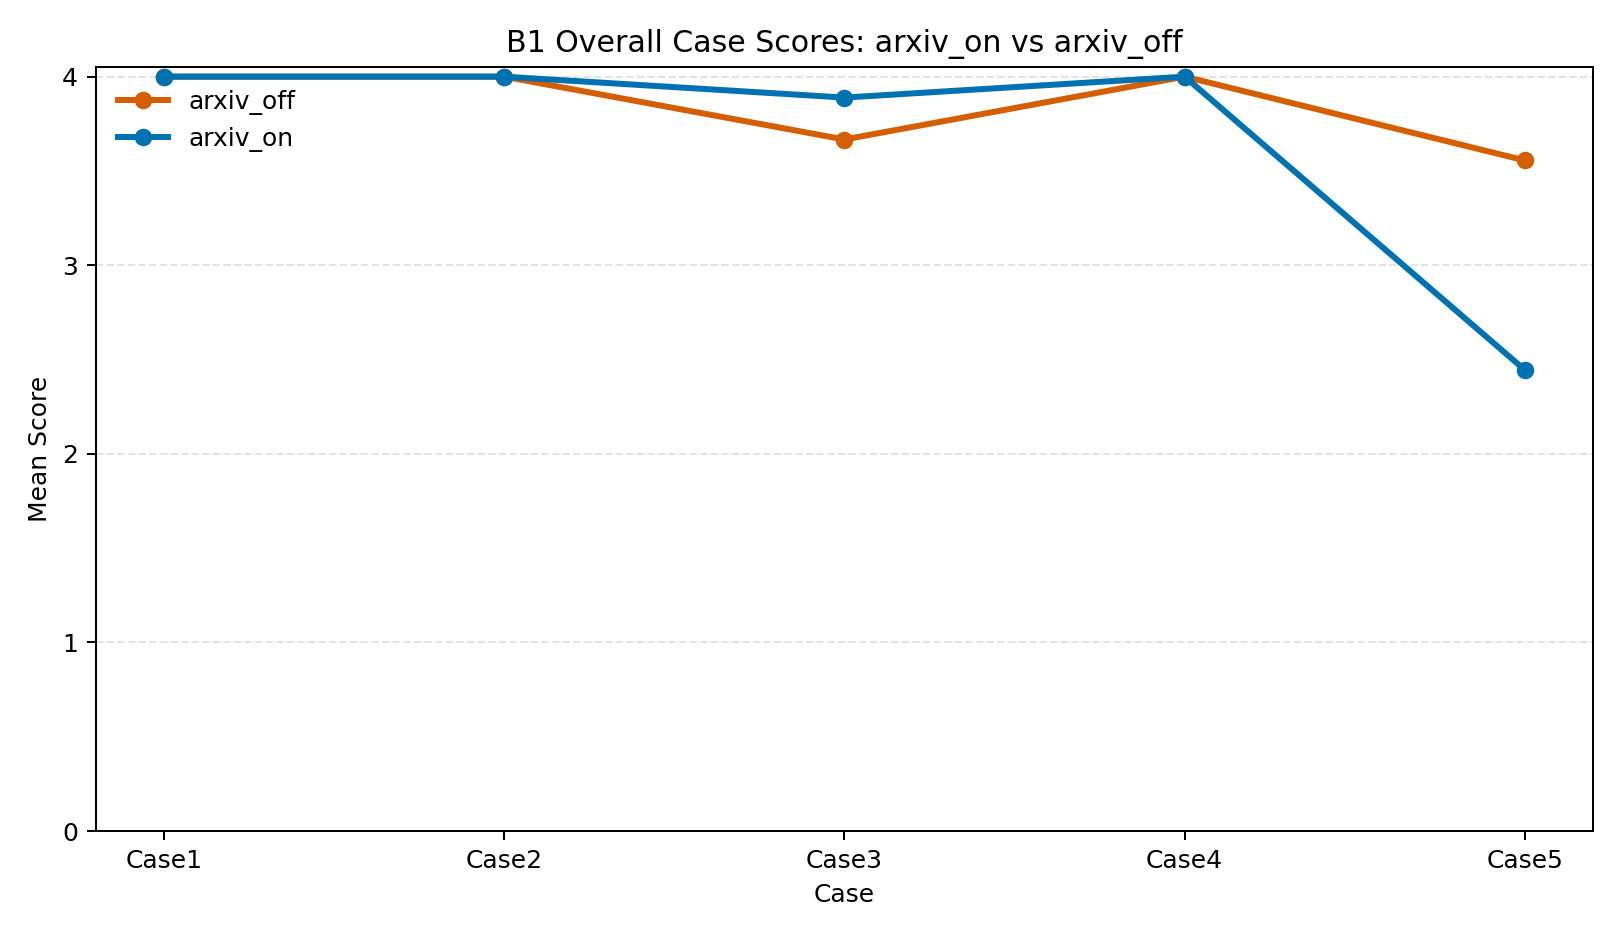
\includegraphics[width=0.48\textwidth,height=0.40\textheight,keepaspectratio]{arxiv-fig1-score-comparison.png}
    \hfill
    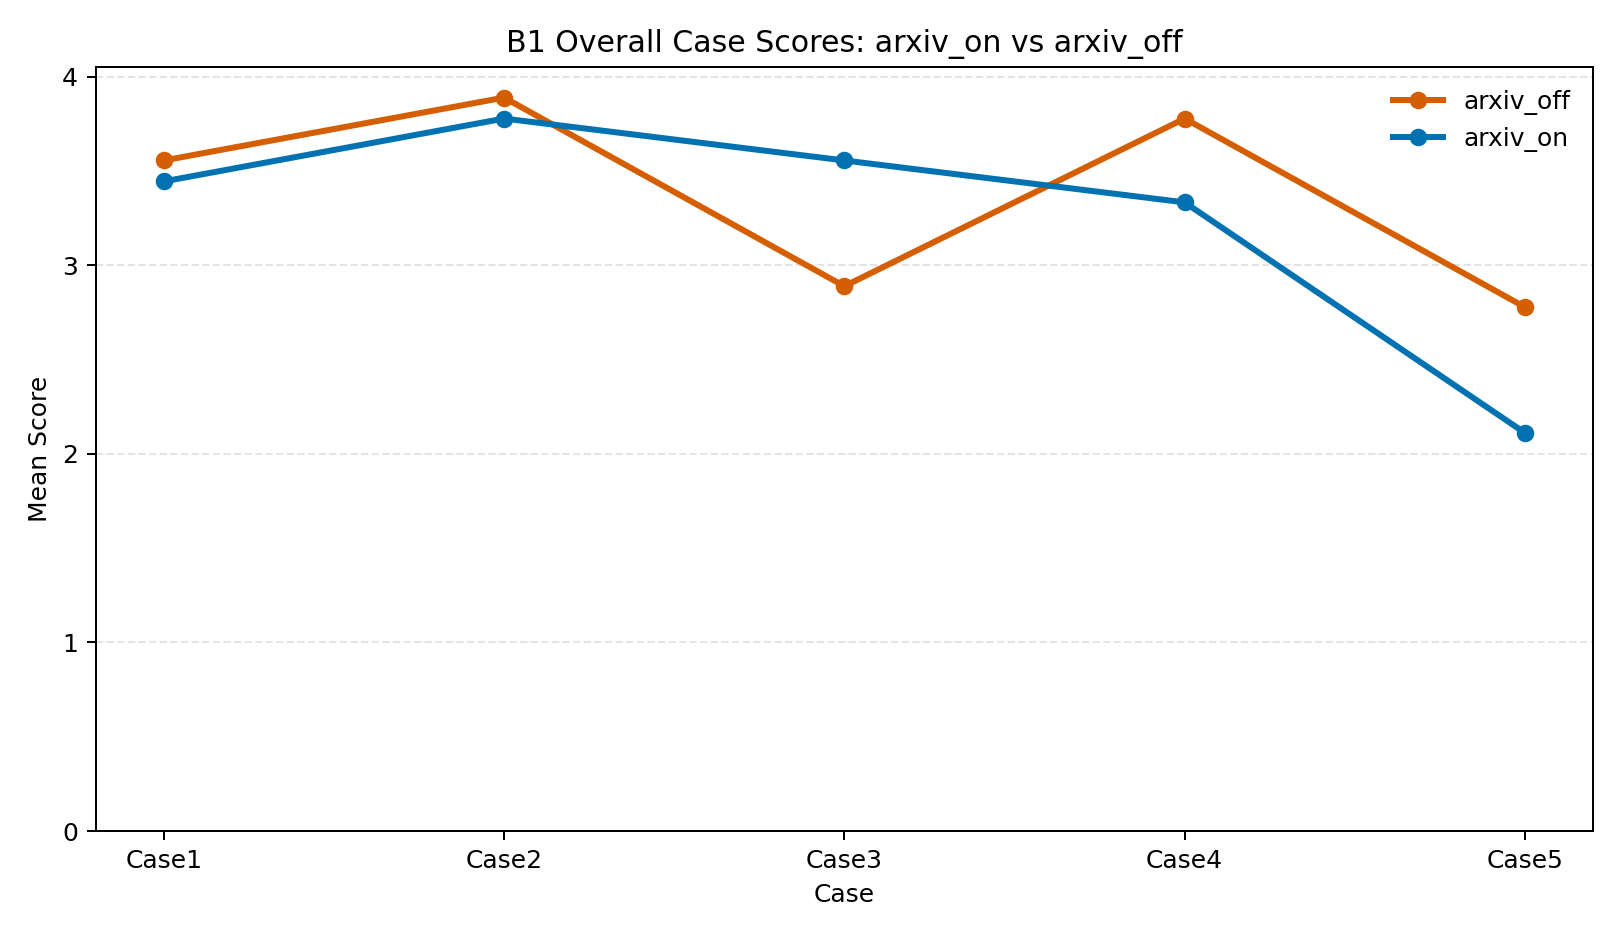
\includegraphics[width=0.48\textwidth,height=0.40\textheight,keepaspectratio]{arxiv-fig2-case-detail.png}

    \vspace{0.2em}
    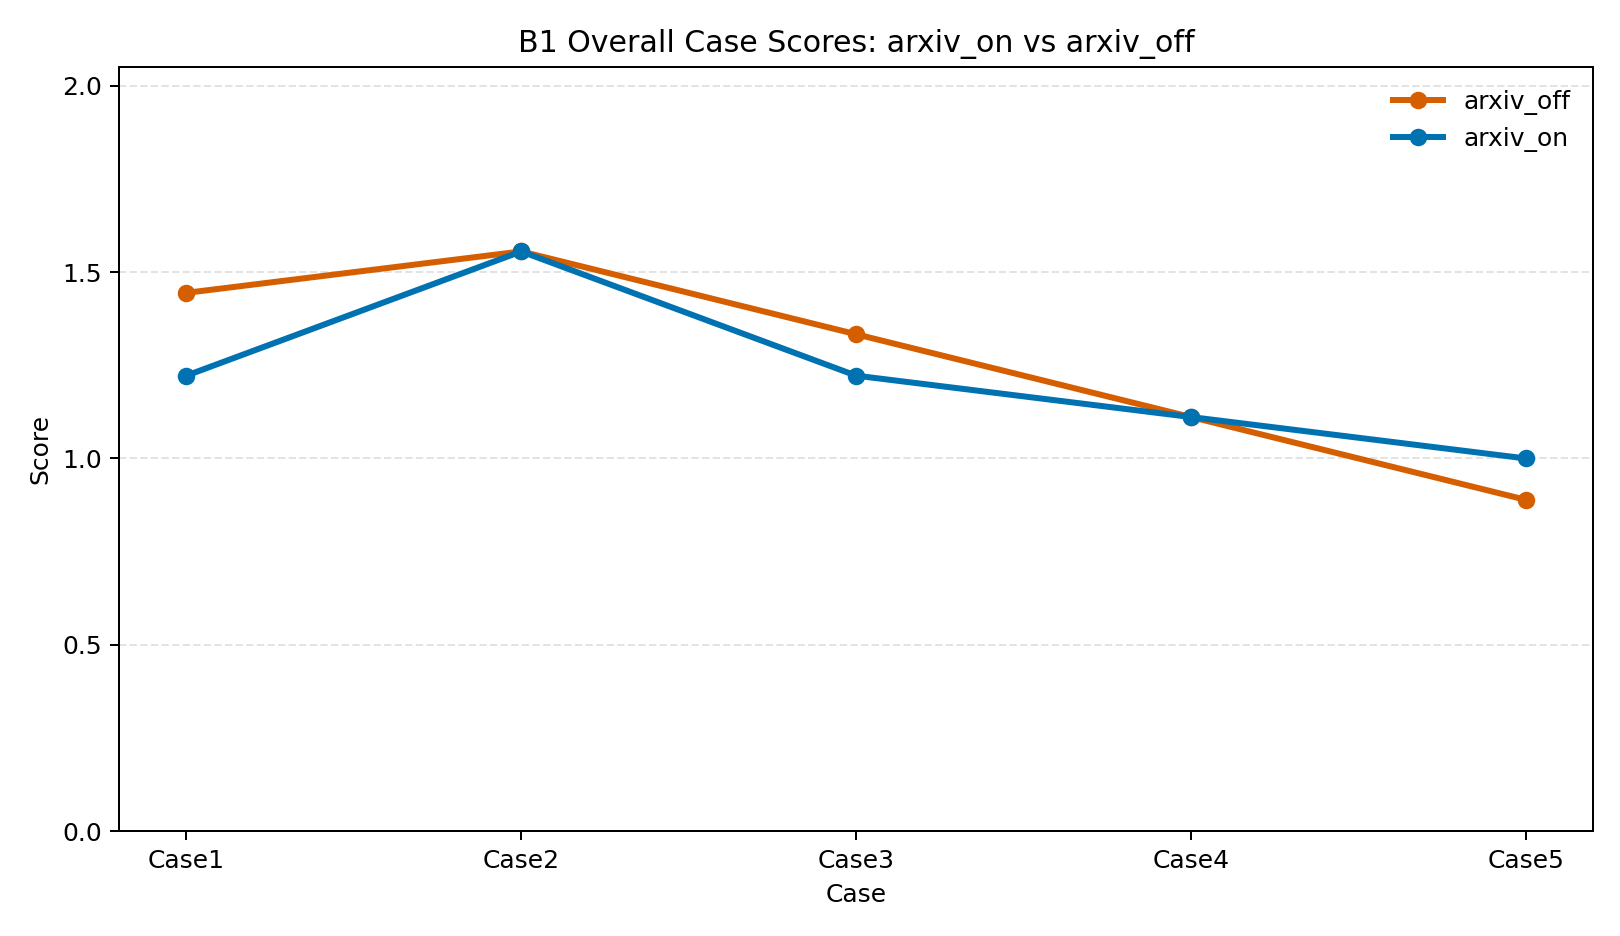
\includegraphics[width=0.70\textwidth,height=0.40\textheight,keepaspectratio]{arxiv-fig3-c5-analysis.png}
  \end{center}
\end{frame}

\begin{frame}{工具预实验 2：refchecker repair}
  \begin{block}{目的}
    测试 mcp-refchecker 是否能作为生成期工具，帮助 Agent 发现并修复引用元数据和部分引用风险。
  \end{block}

  \begin{itemize}
    \item 规模：5 cases $\times$ 3 runs
    \item 每次输出两个报告：原始报告 + repair 后报告
    \item refchecker 负责核查真实出版物/元数据
    \item claim support 仍需要 Agent 读原文并做局部判断
  \end{itemize}

  \vspace{0.4em}
  限制：refchecker 本身不是“语义支持性判定器”，不能替代人工标注。
\end{frame}

\begin{frame}{主实验：Memory MVP}
  \begin{columns}[T,onlytextwidth]
    \begin{column}{0.52\textwidth}
      \begin{block}{运行顺序}
        \begin{itemize}
          \item P1: C1 $\rightarrow$ C2 $\rightarrow$ C3 $\rightarrow$ C4 $\rightarrow$ C5
          \item P2: C1 $\rightarrow$ C2 $\rightarrow$ C3 $\rightarrow$ C4 $\rightarrow$ C5
        \end{itemize}
      \end{block}
    \end{column}
    \begin{column}{0.43\textwidth}
      \begin{block}{Memory 来源}
        \begin{itemize}
          \item 只写入 repair log
          \item 不写入完整报告
          \item 不写入人工标注
          \item 不作为科学证据引用
        \end{itemize}
      \end{block}
    \end{column}
  \end{columns}

  \vspace{0.5em}
  研究目标：观察 Agent 是否能从之前的 refchecker/repair 经验中学到更谨慎的引用行为。
\end{frame}

\begin{frame}{Memory 机制：跨 Case 经验迁移}
  \begin{columns}[T,onlytextwidth]
    \begin{column}{0.52\textwidth}
      \begin{tikzpicture}[node distance=0.4cm and 0.5cm,
        box/.append style={minimum height=0.65cm,font=\footnotesize}]
        \node[box, fill=accentgreen!8, draw=accentgreen, minimum width=2.2cm] (repair) {Case N 完成};
        \node[box, fill=accentgreen!8, draw=accentgreen, below=of repair, minimum width=2.2cm] (extract) {抽取 repair log};
        \node[data, minimum height=0.6cm, font=\footnotesize, below=of extract] (jsonl) {active\_memory.jsonl};
        \node[box, fill=mainblue!8, draw=mainblue, below=of jsonl, minimum width=2.2cm] (retrieve) {词匹配检索 top-6};
        \node[box, fill=accentred!8, draw=accentred, below=of retrieve, minimum width=2.2cm] (next) {Case N+1 运行};

        \draw[arrow] (repair) -- (extract);
        \draw[arrow] (extract) -- (jsonl);
        \draw[arrow] (jsonl) -- (retrieve);
        \draw[arrow] (retrieve) -- (next);
        \draw[arrow] (next.east) to[bend right=25] (repair.east);
      \end{tikzpicture}
    \end{column}
    \begin{column}{0.45\textwidth}
      \begin{block}{写入（Write-back）}
        \begin{itemize}
          \setlength{\itemsep}{2pt}
          \item 来源：\texttt{REFCHECKER\_REPAIR\_LOG} 的 JSONL 行
          \item 包括 clean rows 与 error rows，按 \texttt{memory\_record\_id} 去重
          \item 规范化为摘要、关键词、错误类型、修复动作
          \item \alert{不写入}：完整报告 / 人工标注
        \end{itemize}
      \end{block}
      \vspace{0.2em}
      \begin{block}{检索 + 注入}
        \begin{itemize}
          \setlength{\itemsep}{2pt}
          \item TF-IDF-like 词匹配检索 \textbf{top-6}
          \item 注入为 \texttt{MEMORY\_CONTEXT} procedural caution
          \item \alert{不作为科学证据，不可被引用}
        \end{itemize}
      \end{block}
      \vspace{0.2em}
      \begin{alertblock}{隔离控制}
        每次 case 新 session key，仅通过 JSONL 传递，JOBS=1 顺序执行。
      \end{alertblock}
    \end{column}
  \end{columns}
\end{frame}

\begin{frame}{Memory 实现细节：实际代码路径}
  \small
  \begin{columns}[T,onlytextwidth]
    \begin{column}{0.50\textwidth}
      \begin{block}{Run 前：retrieve}
        \begin{itemize}
          \setlength{\itemsep}{2pt}
          \item 读取共享文件：\texttt{active\_memory.jsonl}
          \item Query = 当前 \texttt{case\_id} + topic + citation/support/refchecker 等关键词
          \item 默认 \texttt{top\_k=6}，context 上限 5000 chars
          \item 输出 \texttt{memory\_context.md}，再拼到 prompt 前面
        \end{itemize}
      \end{block}
    \end{column}

    \begin{column}{0.47\textwidth}
      \begin{block}{Run 后：write-back}
        \begin{itemize}
          \setlength{\itemsep}{2pt}
          \item 只有 marker 完整且无 hard failure 才写回
          \item 抽取 \texttt{\# REFCHECKER\_REPAIR\_LOG} 到 \texttt{\# REPAIRED\_REPORT} 之间的 JSONL
          \item 允许类型：\texttt{reference\_metadata} / \texttt{claim\_citation\_pair}
          \item 当前最终 memory：97 条 records
        \end{itemize}
      \end{block}
    \end{column}
  \end{columns}

  \vspace{0.4em}
  \begin{alertblock}{分析注意}
    \texttt{retrieve\_log.jsonl} 会保留 retry 和调试历史；正式分析应按最终 P1/P2 的 \texttt{run.log} / manifest 过滤。
  \end{alertblock}
\end{frame}

\begin{frame}{可复现材料}
  当前仓库中保留的主要材料：
  \begin{itemize}
    \item prompt 模板与 filled prompts；
    \item OpenClaw profile setup scripts；
    \item preflight audit scripts；
    \item run manifests、run logs、stderr logs、raw outputs；
    \item citation-standard validator；
    \item memory retrieval / writeback scripts；
    \item 后续标注表与统计脚本占位。
  \end{itemize}

  \vspace{0.5em}
  关键原则：报告输出、工具配置、profile、workspace、session key 都要能被追溯。
\end{frame}

\begin{frame}{运行环境与工具链问题}
  \small
  \begin{columns}[T,onlytextwidth]
    \begin{column}{0.49\textwidth}
      \begin{alertblock}{网络与检索层}
        \begin{itemize}
          \setlength{\itemsep}{2pt}
          \item \textbf{arXiv DNS / 代理异常}\\
          Clash Fake-IP 会让 arXiv 解析到异常地址。
          \item \textbf{web search / web fetch timeout}\\
          搜索服务与 arXiv 访问路径不同，代理策略必须分开。
        \end{itemize}
      \end{alertblock}

      \begin{block}{处理}
        固定 \texttt{HTTPS\_PROXY} / \texttt{HTTP\_PROXY}，并用 \texttt{NO\_PROXY} 让 \texttt{arxiv.org} 与 \texttt{export.arxiv.org} 直连。
      \end{block}
    \end{column}

    \begin{column}{0.49\textwidth}
      \begin{alertblock}{MCP 与插件层}
        \begin{itemize}
          \setlength{\itemsep}{2pt}
          \item \textbf{arxiv MCP \texttt{-32000}}\\
          MCP server 手动握手正常，但 OpenClaw bundle-MCP 层偶发连接失败。
          \item \textbf{profile 配置漂移}\\
          DeepSeek auth、Brave provider、memory/session search 可能在新 profile 中不一致。
        \end{itemize}
      \end{alertblock}

      \begin{block}{处理}
        增加 safe wrapper、profile audit 和 manifest；统一 Brave provider，显式关闭非实验变量工具。
      \end{block}
    \end{column}
  \end{columns}
\end{frame}

\begin{frame}{工具链问题如何约束实验设计}
  \scriptsize
  \begin{tabularx}{\textwidth}{@{}p{0.22\textwidth}XX@{}}
    \toprule
    工程风险 & 若不控制会怎样 & 实验中的控制方式 \\
    \midrule
    并行运行不稳定 &
    \texttt{JOBS=2} 放大 arXiv、web search、DeepSeek API timeout，失败和模型能力混在一起。 &
    主实验固定 \texttt{JOBS=1}；失败 run 保留日志并用新 session key 重试。 \\
    workspace / memory 污染 &
    下载论文、临时文件、聊天历史和 memory 写回跨 run 泄漏，破坏变量隔离。 &
    预实验独立 profile / workspace；Memory 只在 \texttt{M1\_memory\_on} 内按 C1--C5 顺序共享。 \\
    输出格式漂移 &
    自由文本引用位置无法稳定解析，claim--citation pair 抽取不可复现。 &
    固定四段 marker；开启 citation-standard skill；validator 检查 CPS 格式。 \\
    工具能力边界不清 &
    arxiv MCP 或 refchecker 的基础设施问题可能被误判为 Agent 推理能力差异。 &
    先做工具预实验；主实验只解释在固定工具栈下的引用一致性表现。 \\
    \bottomrule
  \end{tabularx}

  \vspace{0.35em}
  \begin{alertblock}{复现边界}
    prompt + profile audit + run manifest + stderr + raw output + memory snapshot + pass-specific papers。
  \end{alertblock}
\end{frame}

\begin{frame}{refchecker Repair 效果：LLM 评测结果}
  \begin{block}{评测方式：\texttt{citation\_check} 流水线}
    人工定义错误分类体系 + 编写 few-shot prompt → \texttt{build\_judge\_inputs.py} 抽取 claim–citation pair 并构造 batch → \texttt{run\_deepseek\_judge.py} 送入 DeepSeek 批量判定。5 cases $\times$ 3 runs $\times$ repair yes/no，按 run 取均值 ± std。
  \end{block}

  \vspace{-0.5em}
  \begin{columns}[T,onlytextwidth]
    \begin{column}{0.55\textwidth}
      \begin{center}
        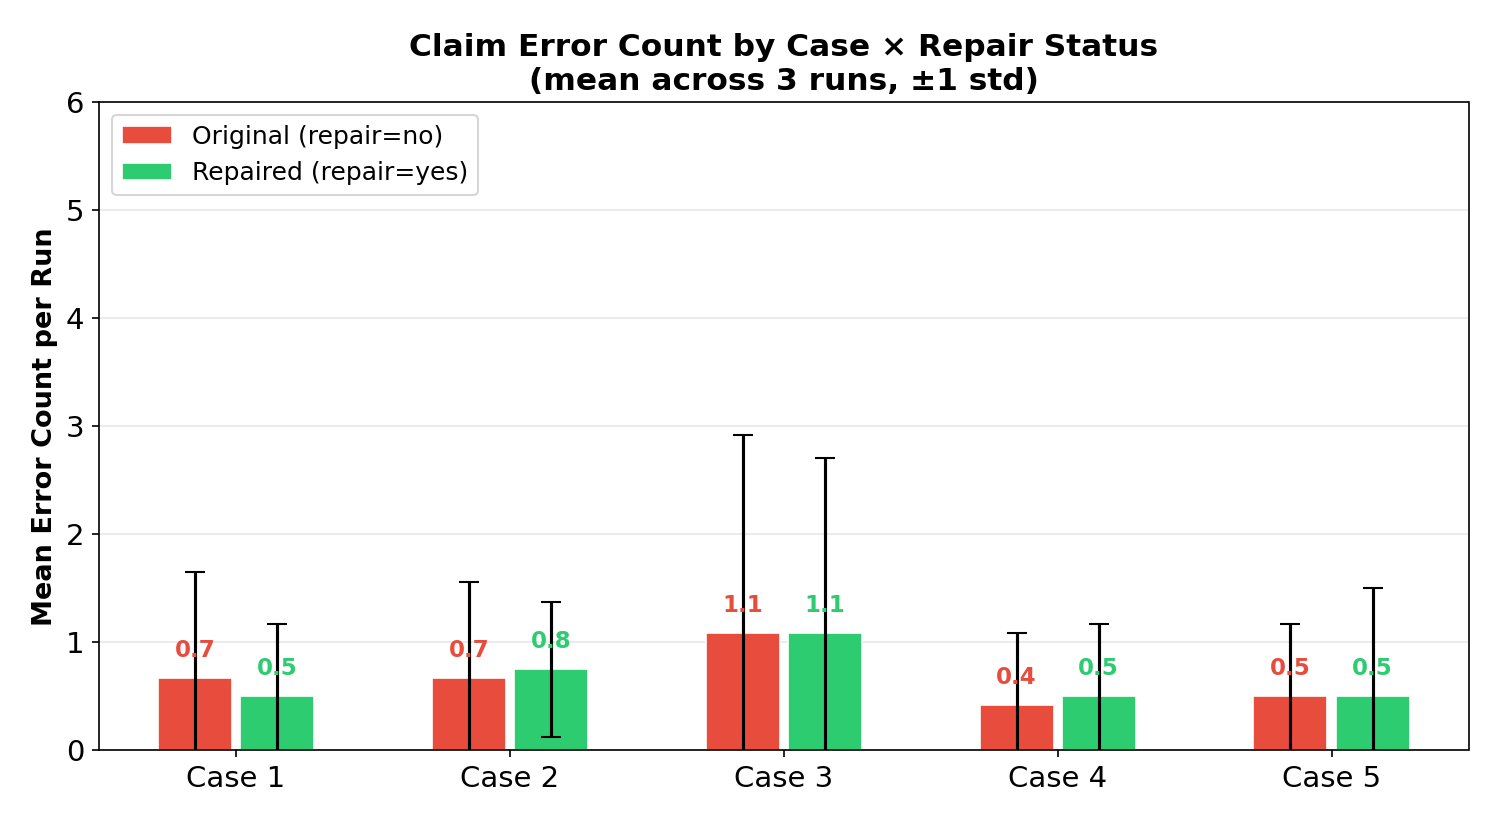
\includegraphics[width=0.93\textwidth]{repair_effect_summary.png}
      \end{center}
    \end{column}
    \begin{column}{0.42\textwidth}
      \begin{alertblock}{核心结论}
        \begin{itemize}
          \setlength{\itemsep}{3pt}
          \item 总错误量：40 → 40\\\alert{repair 没有减少错误总量}
          \item 只有 \textbf{C1} 有改善（8→6）
          \item C2、C4 repair 后反而增加
          \item C3、C5 完全持平
        \end{itemize}
      \end{alertblock}
    \end{column}
  \end{columns}
\end{frame}

\begin{frame}{错误类型分布：2×2 全景}
  \begin{center}
    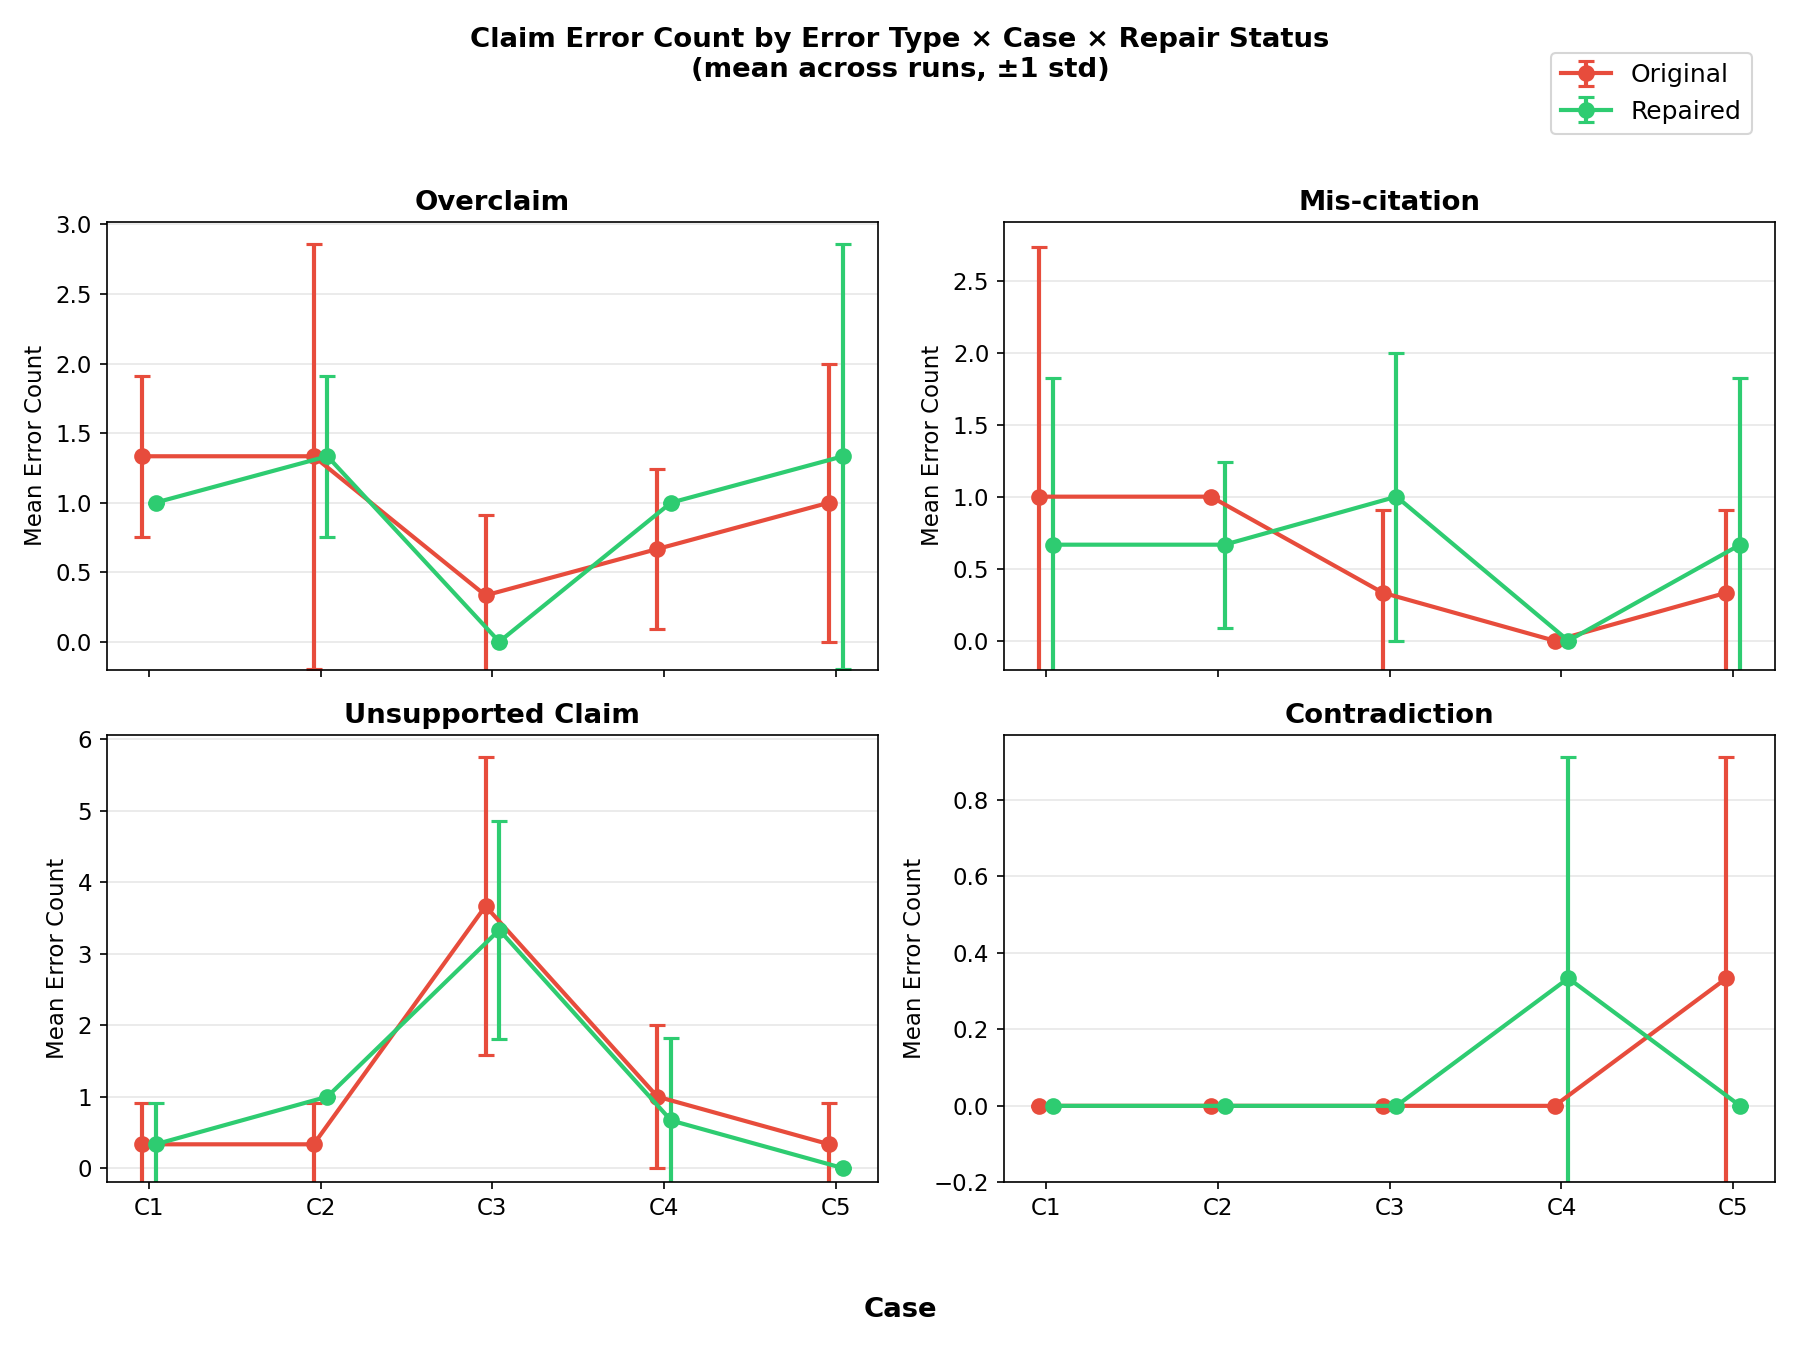
\includegraphics[width=0.92\textwidth,height=0.78\textheight,keepaspectratio]{error_rate_by_type.png}
  \end{center}
\end{frame}

\begin{frame}{错误类型分布：关键发现}
  \begin{alertblock}{C3 的 Unsupported Claim 是绝对主力（85\%）}
    \begin{itemize}
      \item C3（蛋白-配体 docking）Unsupported Claim 均值 3.3--3.7，远超其他所有类型
      \item repair 前后几乎不变：11 → 10 个
      \item 这类 claim 元数据完全正确，但语义支撑不成立
    \end{itemize}
  \end{alertblock}

  \vspace{0.3em}
  \begin{block}{根源：refchecker 的能力边界}
    \begin{center}
    \begin{tabular}{p{0.43\textwidth}|p{0.43\textwidth}}
      \textbf{refchecker 能做的} & \textbf{refchecker 不能做的} \\
      \hline
      验证论文是否存在 & 判断结论是否被引用支撑 \\
      核对作者/标题/年份 & 评估专业领域的证据强度 \\
      检查 DOI / arXiv ID & 发现“听起来科学但无定量支撑”的 claim \\
    \end{tabular}
    \end{center}
  \end{block}

  \textbf{Citation verification $\neq$ Claim verification} —— 领域越专业，语义支撑判断越需要领域 expertise，refchecker 越无能为力。
\end{frame}

\begin{frame}{Failure Case 实例}
  \begin{block}{Case A: Mis-citation — 引用沾边但接不上}
    \begin{enumerate}
      \setlength{\itemsep}{4pt}
      \item \textbf{C1 (SWE-Bench)}：“精心设计的 agent-computer interface 是将 LLM 转化为高效编码 agent 的关键，直接使用 vanilla shell 交互会导致性能大幅下降。”
      \\→ 被引论文主题相关，但讨论的是另一个对象/任务，引用位置无法支撑该具体论断。

      \item \textbf{C2 (Model Collapse)}：“仅在合成数据上递归训练的统计语言模型会发生完全塌缩，学到的条件分布以概率 1 收敛至 Dirac 分布。”
      \\→ 沾边但实际讨论条件不同，属于“听起来像但实际不是”。

      \item \textbf{C5 (AI Coding)}：“开发者编码经验不预测 AI 工具采纳率，但显著影响其对 AI 角色的心理模型。”
      \\→ 引用定位错误，被引论文的结论范围与此 claim 不匹配。
    \end{enumerate}
  \end{block}
\end{frame}

\begin{frame}{Failure Case 实例（续）}
  \begin{block}{Case B: Overclaim — 结论强于原文证据}
    \begin{enumerate}
      \setlength{\itemsep}{2pt}
      \item \textbf{C1}: “工具增强型 LLM agent 的 Pass@1 可从 17\% 提升至 53\%。” → 把单次实验数值夸大为普遍结论，忽略实验设定局限。
      \item \textbf{C4}: “MLLM 在透视感知中存在系统性缺陷，与人类差距显著。” → 将有限 benchmark 的观测推广为“系统性缺陷”。
      \item \textbf{C5}: “AI 更适合辅助而非替代有经验的工程师。” → 原文仅有用户反馈分析，并未设计对照实验支撑强因果结论。
    \end{enumerate}
  \end{block}

  \vspace{0.1em}
  \begin{alertblock}{Case B: Contradiction — 罕见但最严重}
    \begin{enumerate}
      \setlength{\itemsep}{1pt}
      \item \textbf{C5}: “使用 AI 后任务时间延长约 32\%” — 原文部分数据指向效率提升，方向相反。
      \item \textbf{C4}: “异构物体组合引发更严重幻觉，GPT-4o 也不例外” — 被引论文结论方向与该表述冲突。
    \end{enumerate}
  \end{alertblock}
\end{frame}

\begin{frame}{Repair 的本质：错误类型漂移，而非消除}
  \begin{block}{20 个配对 claim 中，7 个在 repair 后错误类型改变}
    \begin{tabularx}{\textwidth}{@{}lccX@{}}
      \toprule
      变化方向 & 次数 & 是好是坏？ & 含义 \\
      \midrule
      Overclaim → Mis-citation & 2 & 不确定 & 措辞弱化了，但引用位置错了 \\
      Mis-citation → Overclaim & 2 & 变差 & 引用修对了，但表述夸大了 \\
      Mis-citation → Unsupported Claim & 1 & 暴露问题 & 引用修对后，证据不足被暴露 \\
      Contradiction → Overclaim & 1 & 不确定 & 矛盾消除了，但变成了夸大 \\
      Unsupported Claim → Mis-citation & 1 & 不确定 & 加了引用，但引错了 \\
      \bottomrule
    \end{tabularx}
  \end{block}

  \vspace{0.3em}
  \begin{alertblock}{Agent 基于 refchecker 反馈改写时，缺乏对原文证据的深入理解}
    改写方向是\alert{随机的}——有时变好，有时变差，有时只是换了一种错法。
    Repair 的 prompt 目标应该是\alert{消除错误}，而非仅仅是改写。
  \end{alertblock}
\end{frame}

\begin{frame}{归因分析总结}
  \begin{enumerate}
    \item \textbf{refchecker 解决的是引用真实性，不是引用支撑性}\\
    \quad → C3 Unsupported Claim repair 前后: 11 → 10，几乎无效

    \item \textbf{repair 效果与 Agent 对领域的先验知识正相关}\\
    \quad → 只有 C1（最主流 CS topic）有改善

    \item \textbf{repair 是错误类型漂移，不是错误消除}\\
    \quad → 7/20 claim 错误类型改变，总错误量不变（40→40）

    \item \textbf{领域专业度越高，repair 越无效}\\
    \quad → C3（生化）完全无效，C1（CS）轻微有效

    \item \textbf{Unsupported Claim 是当前系统最致命的盲区}\\
    \quad → 占总错误 46\%，且 repair 完全无法解决
  \end{enumerate}

  \vspace{0.4em}
  \begin{block}{改进方向}
    面向 source-grounded check 升级；高专业度 case 采用更保守的 claim 策略；repair 改为“改写→再核查→再改写”迭代循环。
  \end{block}
\end{frame}

% ================================================================
%  Memory 实验结果
% ================================================================

\begin{frame}{Memory 实验：M1 错误总数（per run）}
  \begin{columns}[T,onlytextwidth]
    \begin{column}{0.55\textwidth}
      \begin{center}
        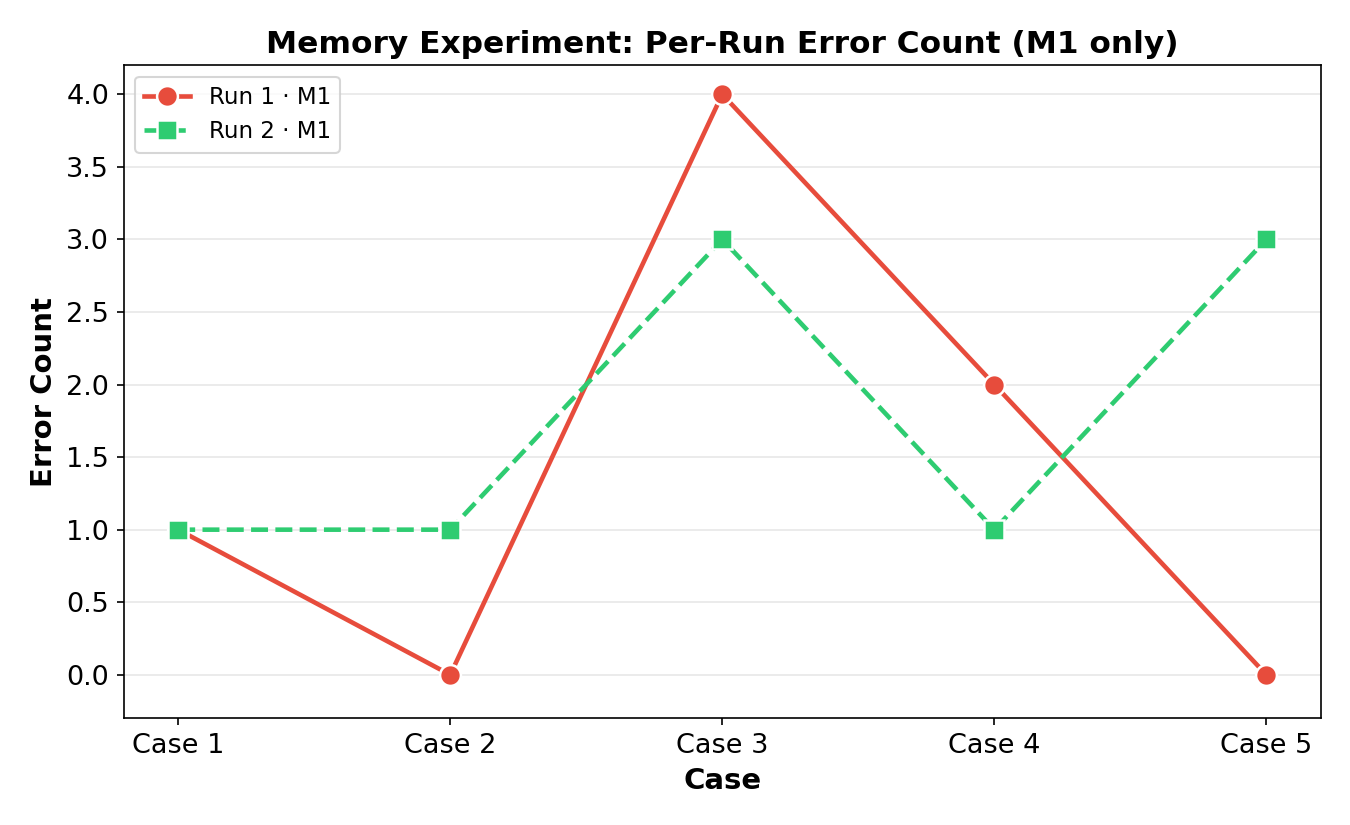
\includegraphics[width=\textwidth]{memory_by_run.png}
      \end{center}
    \end{column}
    \begin{column}{0.42\textwidth}
      \begin{block}{实验设置}
        \begin{itemize}
          \setlength{\itemsep}{3pt}
          \item M1 = memory on（只注入 repair log）
          \item 5 cases $\times$ 2 runs
          \item LLM 逐 claim 错误分类
        \end{itemize}
      \end{block}
      \vspace{0.3em}
      \begin{alertblock}{关键发现}
        \begin{itemize}
          \setlength{\itemsep}{3pt}
          \item \textbf{C1 错误数最低}（R1=1, R2=1）
          \item \textbf{C3 最高}（R1=4, R2=3），两 run 一致
          \item C5 两 run 差异大（0 vs 3）
        \end{itemize}
      \end{alertblock}
    \end{column}
  \end{columns}
\end{frame}

\begin{frame}{Memory 实验：分错误类型（M1 only）}
  \begin{center}
    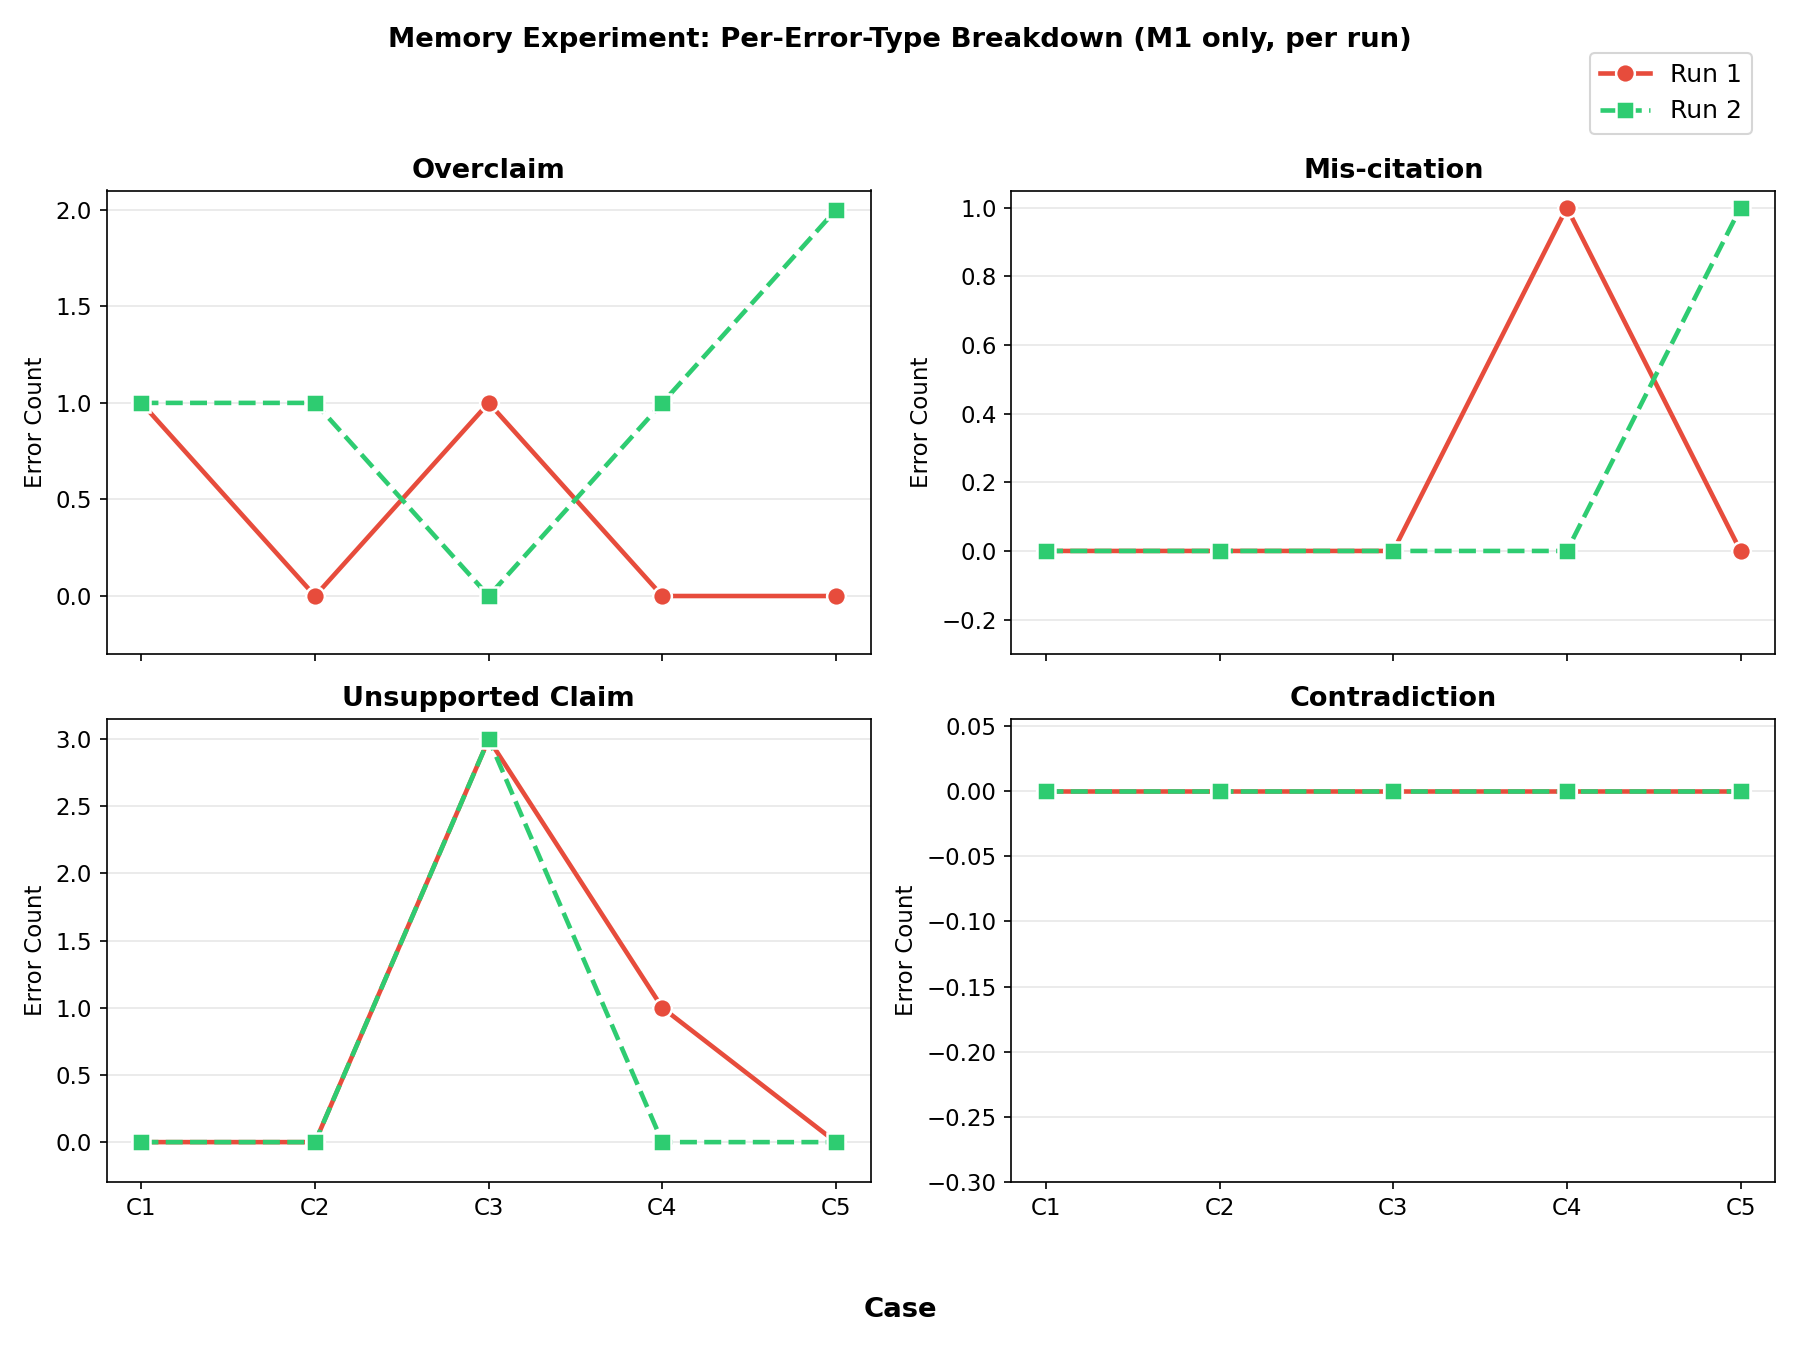
\includegraphics[width=0.88\textwidth,height=0.80\textheight,keepaspectratio]{memory_by_type.png}
  \end{center}
\end{frame}

\begin{frame}{Memory 实验：分错误类型分析}
  \begin{block}{Overclaim — 两个 run 分布不一致}
    \begin{itemize}
      \setlength{\itemsep}{2pt}
      \item Run1: C1=1, C3=1，其余为 0（较干净）
      \item Run2: C5=2（最多），C1/C2/C4 各 1
      \item 两 run 的 C5 差异最大：0 vs 2
    \end{itemize}
  \end{block}

  \vspace{0.3em}
  \begin{block}{Unsupported Claim — 全集中在 C3}
    \begin{itemize}
      \setlength{\itemsep}{2pt}
      \item C3 两 run 各 3 个（占总 Unsupported Claim 的 100\%）
      \item 蛋白-配体领域的定量 claim 即使有 memory 也依然无法验证语义支撑
    \end{itemize}
  \end{block}

  \vspace{0.3em}
  \begin{alertblock}{好消息}
    \textbf{Contradiction 清零} — memory 条件下两个 run 都没有出现矛盾型错误。Mis-citation 也极少（R1: C4=1; R2: C5=1）。
  \end{alertblock}
\end{frame}

\begin{frame}{Memory vs Refchecker：效果对比}
  \vspace{-0.3em}
  \begin{center}
    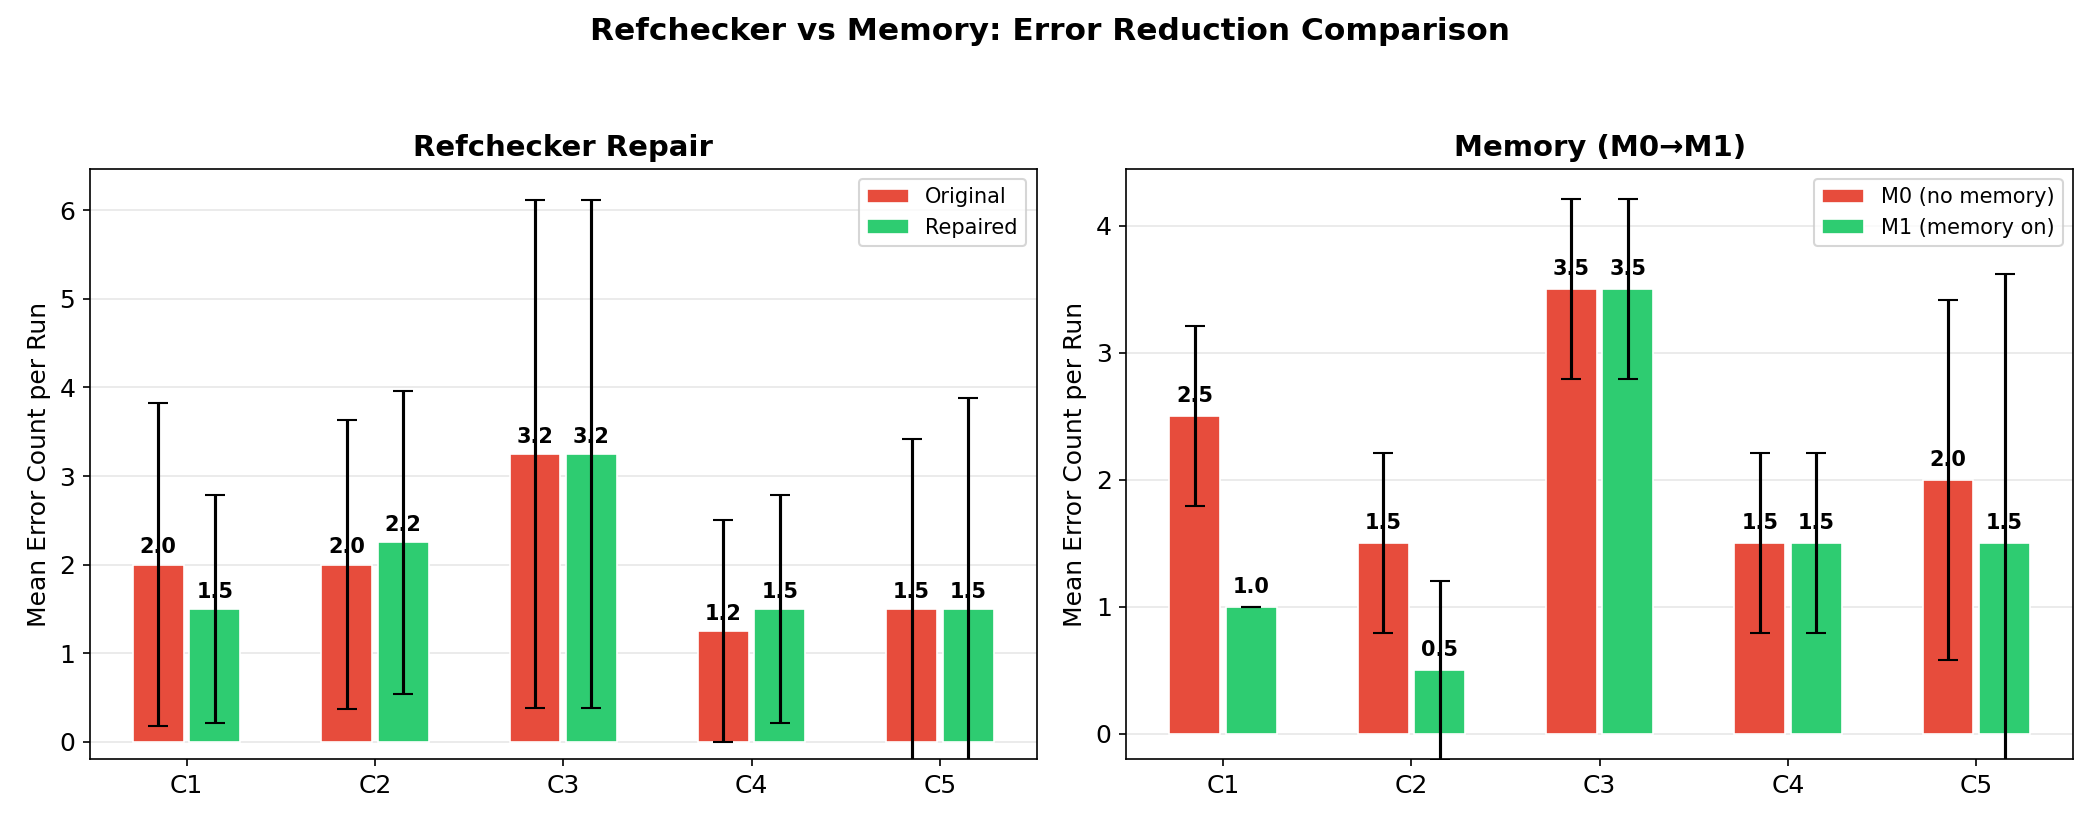
\includegraphics[width=0.72\textwidth]{memory_vs_refchecker.png}
  \end{center}

  \vspace{-0.2em}
  \begin{columns}[T,onlytextwidth]
    \begin{column}{0.48\textwidth}
      \begin{block}{Refchecker Repair}
        \begin{itemize}
          \setlength{\itemsep}{1pt}
          \item 总错误 40→40（无变化）
          \item 只 C1 轻微改善
          \item 错误类型漂移，非消除
        \end{itemize}
      \end{block}
    \end{column}
    \begin{column}{0.48\textwidth}
      \begin{block}{Memory (M1)}
        \begin{itemize}
          \setlength{\itemsep}{1pt}
          \item 总错误 22→16（-27\%）
          \item C1 + C2 均改善
          \item 真正的错误减少
        \end{itemize}
      \end{block}
    \end{column}
  \end{columns}
\end{frame}

\begin{frame}{Memory 归因分析}
  \begin{enumerate}
    \setlength{\itemsep}{6pt}
    \item \textbf{Memory 比 refchecker repair 更有效}\\
    \quad → Memory 减少的是重复犯错（Agent 学到之前的教训），refchecker 只做元数据检查

    \item \textbf{Memory 帮助最大的是主流 CS 领域（C1, C2）}\\
    \quad → Agent 能从 SWE-Bench / model collapse 的 repair log 中提取可迁移经验

    \item \textbf{Memory 对 C3（生化）完全无效}\\
    \quad → Unsupported Claim 6/6 全在 C3，memory 无法弥补领域知识鸿沟

    \item \textbf{Memory 消除了 Contradiction（最严重错误类型）}\\
    \quad → 说明 Agent 从之前 case 的 repair 中学到了“不要和原文对着干”

    \item \textbf{C5 两 run 差异大，提示 memory 效果不稳定}\\
    \quad → Run1=0, Run2=3，可能与 C5 自身论文分布广、Agent 检索差异有关
  \end{enumerate}
\end{frame}

\begin{frame}{初步经验}
  \begin{itemize}
    \item 科研 Agent 的引用问题不只是“有没有引用”，而是“引用是否真的能支撑结论”；
    \item 工具链可用性本身需要预实验验证，否则主实验会被基础设施噪声污染；
    \item citation 格式标准化是后续评测自动化的前提；
    \item refchecker 对元数据有帮助，但 claim support 仍需要 source-grounded 判断；
    \item memory 实验必须严格控制顺序和写入来源，否则很容易引入不可解释的混杂。
  \end{itemize}
\end{frame}

\begin{frame}{一句话总结}
  \begin{center}
    \Large
    我们把“科研 Agent 是否会用看似可靠的引用支撑不可靠结论”\\
    转化为一个可复现、可标注、可消融的 OpenClaw 评测流程。
  \end{center}

  \vspace{1em}
  \begin{center}
    \normalsize
    当前重点不是先证明某个错误率，而是先把实验脚手架、工具控制、输出格式和日志链路固定下来。
  \end{center}
\end{frame}

\end{document}
